% Document Styling
\documentclass[12pt]{article}
\usepackage[margin=1in]{geometry}
\usepackage{graphicx}
\graphicspath{{images/}}
\usepackage{booktabs}
\usepackage[colorlinks=true,linkcolor=black,anchorcolor=black,citecolor=black,filecolor=black,menucolor=black,runcolor=black,urlcolor=black]{hyperref}

\begin{document}

\title{EE 374N Homework 2}
\author{Ishan Shah}
\date{\today}
\maketitle

\section{Signal Processing}
We'll start by plotting subject 1's raw signals for run 1. This was a Point movement.

\begin{center}
    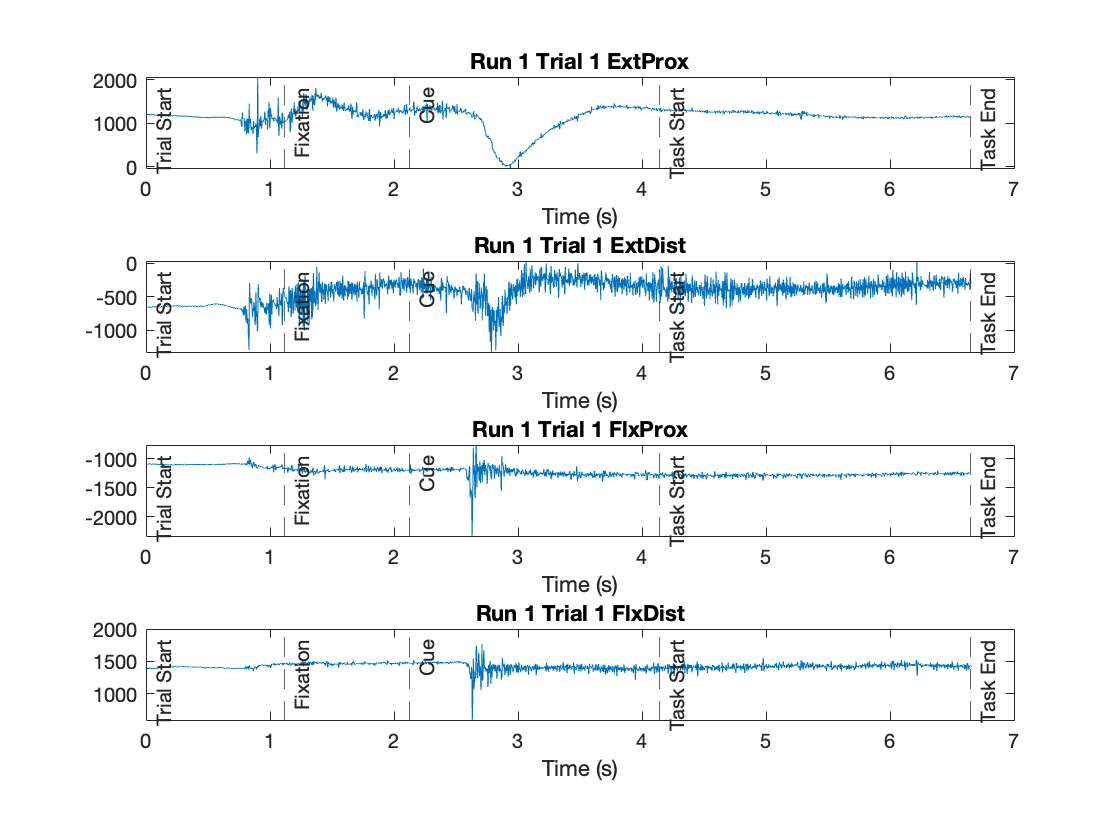
\includegraphics[width=0.8\textwidth]{raw_signals.png}
\end{center}

Now, we can extract the rest and task periods and plot the PSDs for each signal. We can see that the 40-90 Hz band is the most discriminative for the task period.

\begin{center}
    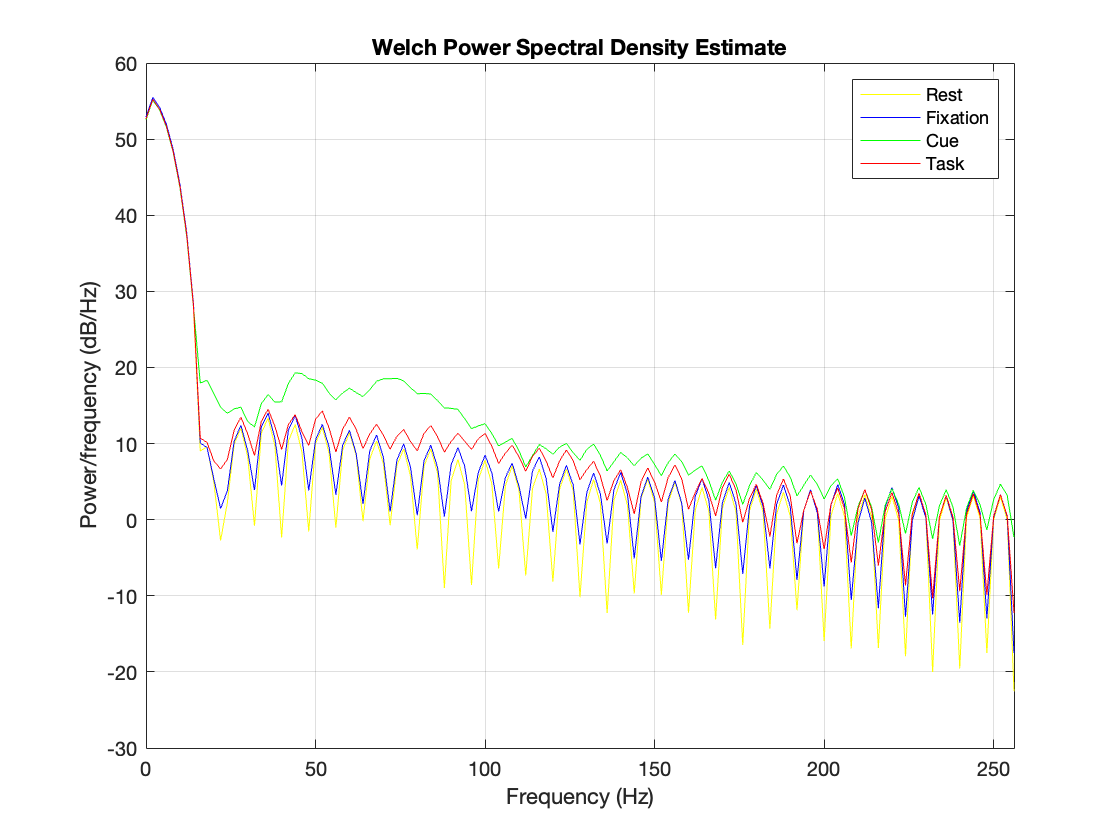
\includegraphics[width=0.8\textwidth]{raw_welch.png}
\end{center}

By filtering by this frequency band, we can see that the task period is much more distinct.

\begin{center}
    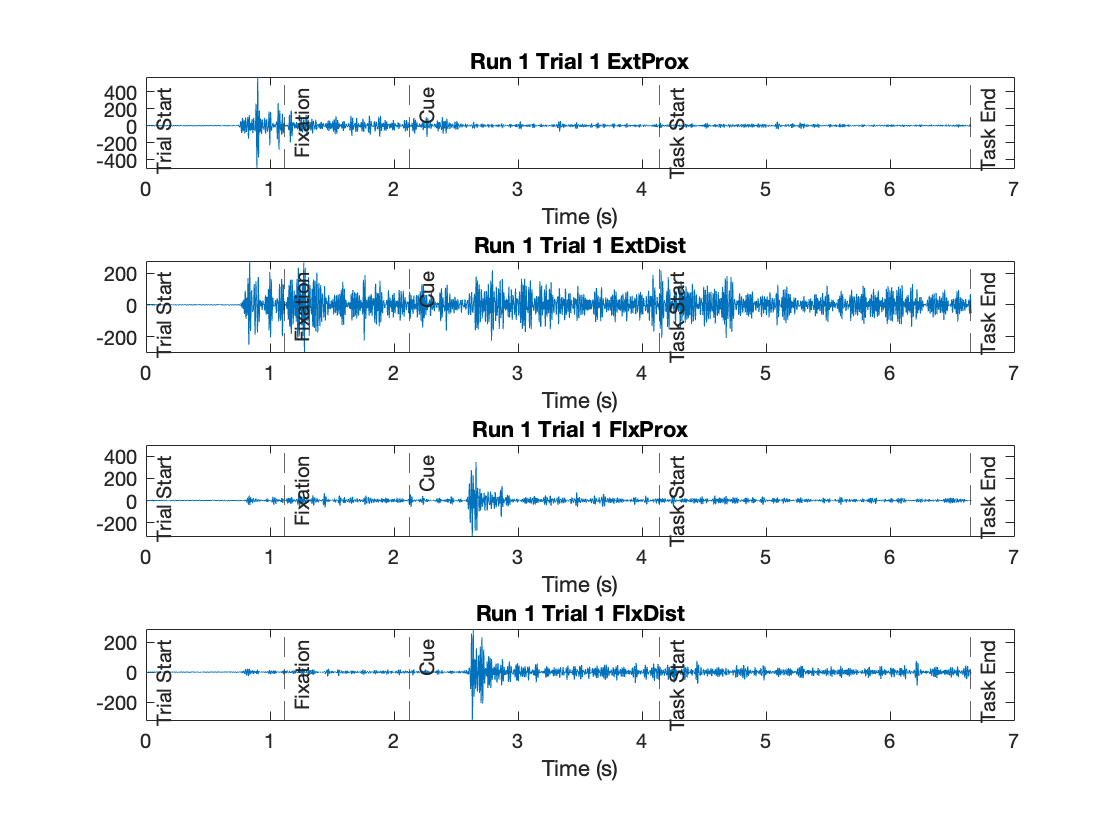
\includegraphics[width=0.8\textwidth]{filtered_signals.png}
\end{center}

\begin{center}
    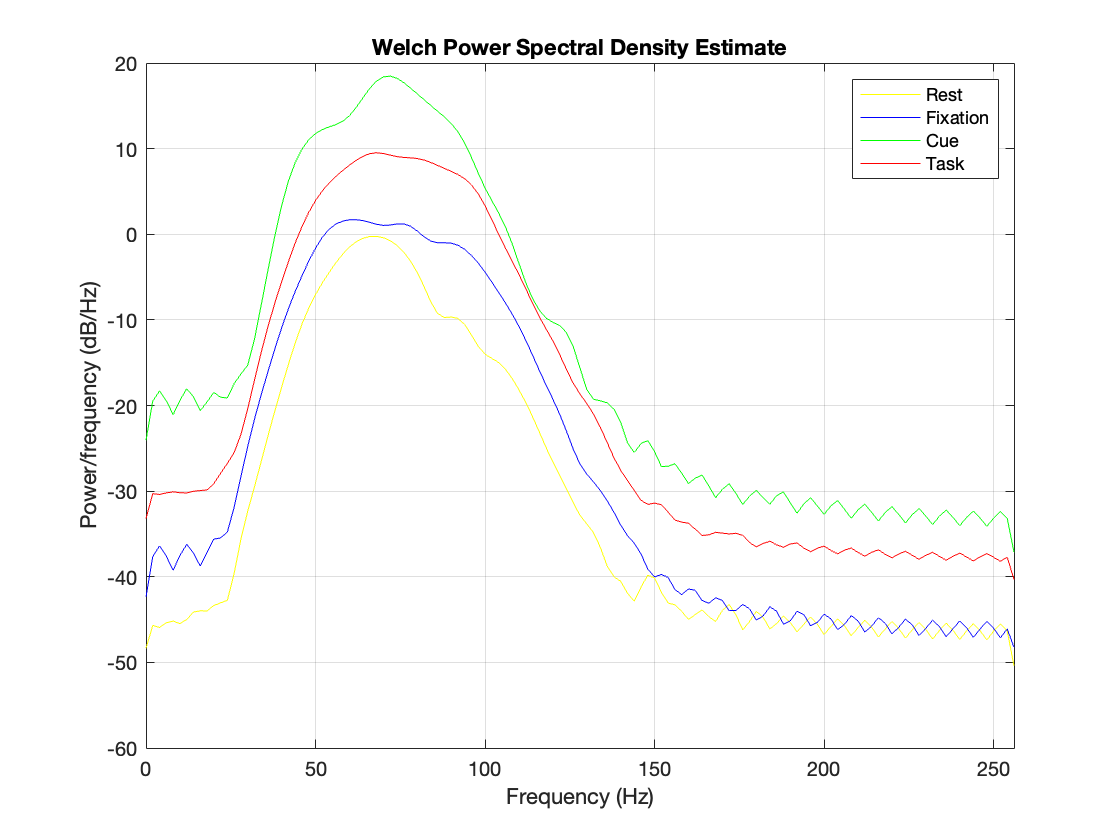
\includegraphics[width=0.8\textwidth]{filtered_welch.png}
\end{center}

\section{Feature Extraction}
I chose to implement the MAV feature and the Waveform Length (WL) feature as I found them used in some literature on EMG-based classification (\url{https://www.sciencedirect.com/science/article/pii/S1877050915038478}) and they seemed to be relatively easy to implement. WL is the length of the signal task computed by summing the absolute differences between adjacent samples. Now we can plot these features for each of the four sensors by subject.

\begin{center}
    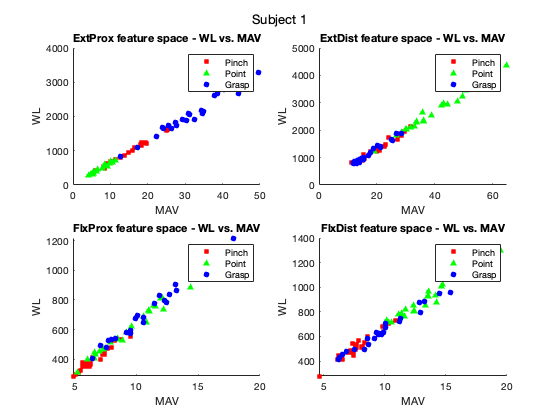
\includegraphics[width=0.9\textwidth]{subject1.png}
\end{center}

\begin{center}
    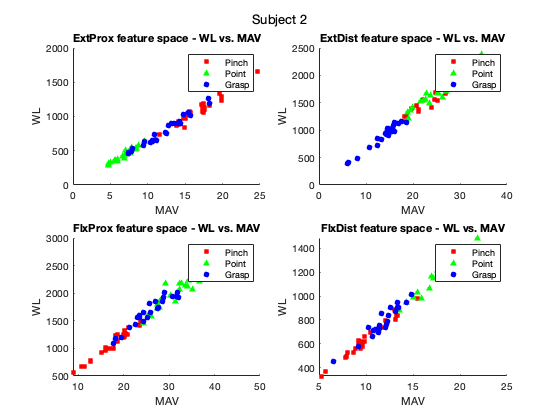
\includegraphics[width=0.9\textwidth]{subject2.png}
\end{center}

These plots tell us that there is a strong linear correlation between WL and MAV for both subjects. ExtProx looks easier to use for classification since it appears more separable than other sensors like FlxDist.

\section{Average Patterns}

Finally, we can plot the average patterns across trials for MAV. We see that the average trial is very smooth compared to the randomly chosen trials and that averaging is a powerful tool for smoothing out noise. Also, the average patterns with MAV are better than the features shown in the previous exercise as they are more constant which makes them more useful.

\begin{center}
    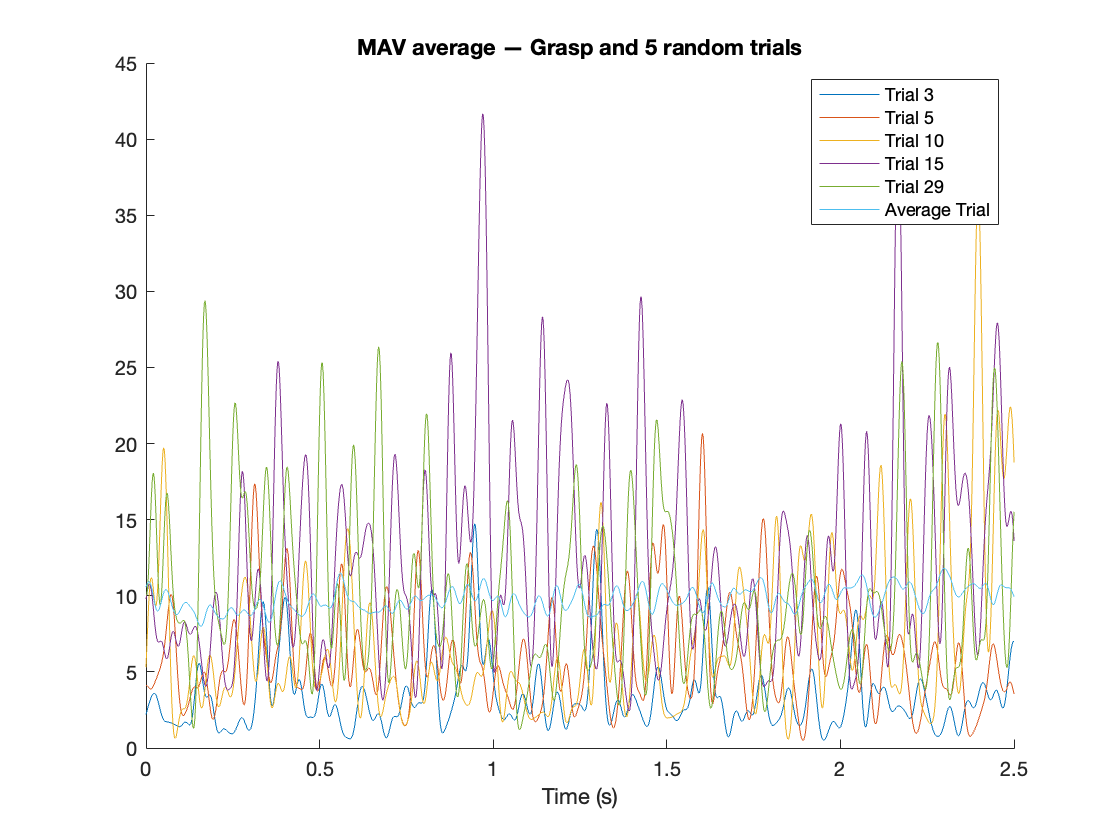
\includegraphics[width=0.9\textwidth]{grasp.png}
\end{center}

\begin{center}
    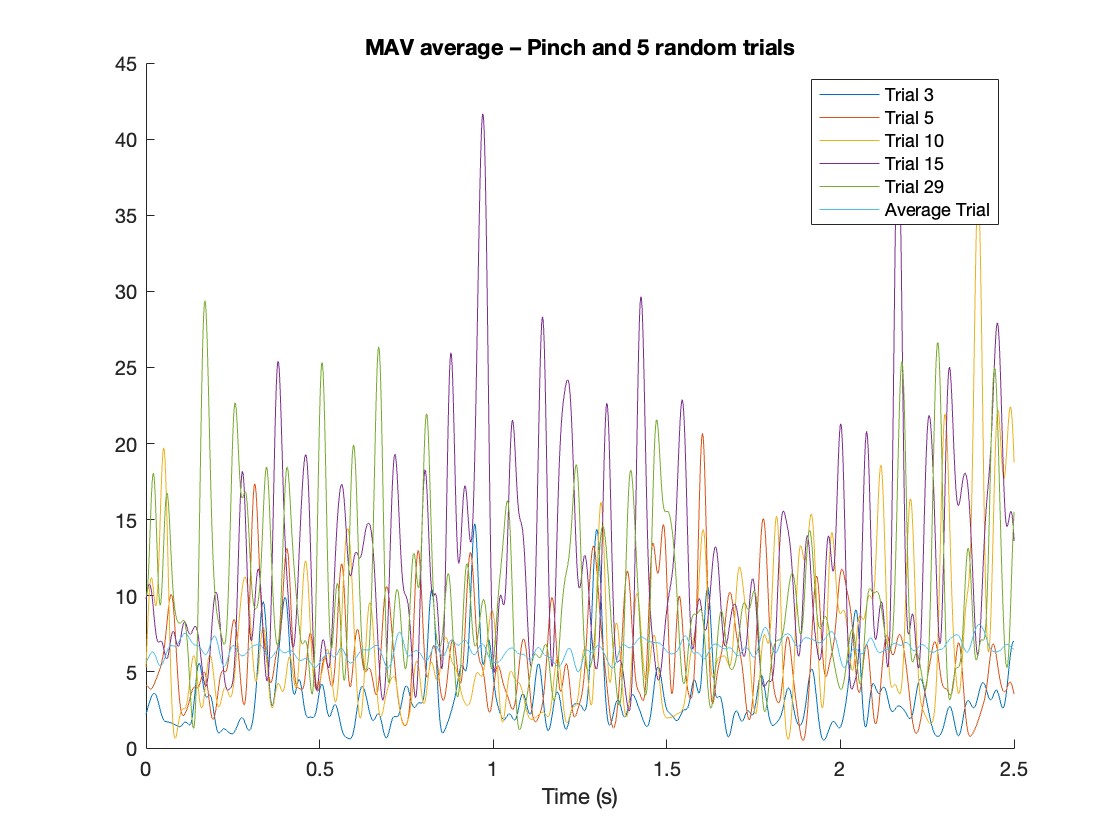
\includegraphics[width=0.9\textwidth]{pinch.png}
\end{center}

\begin{center}
    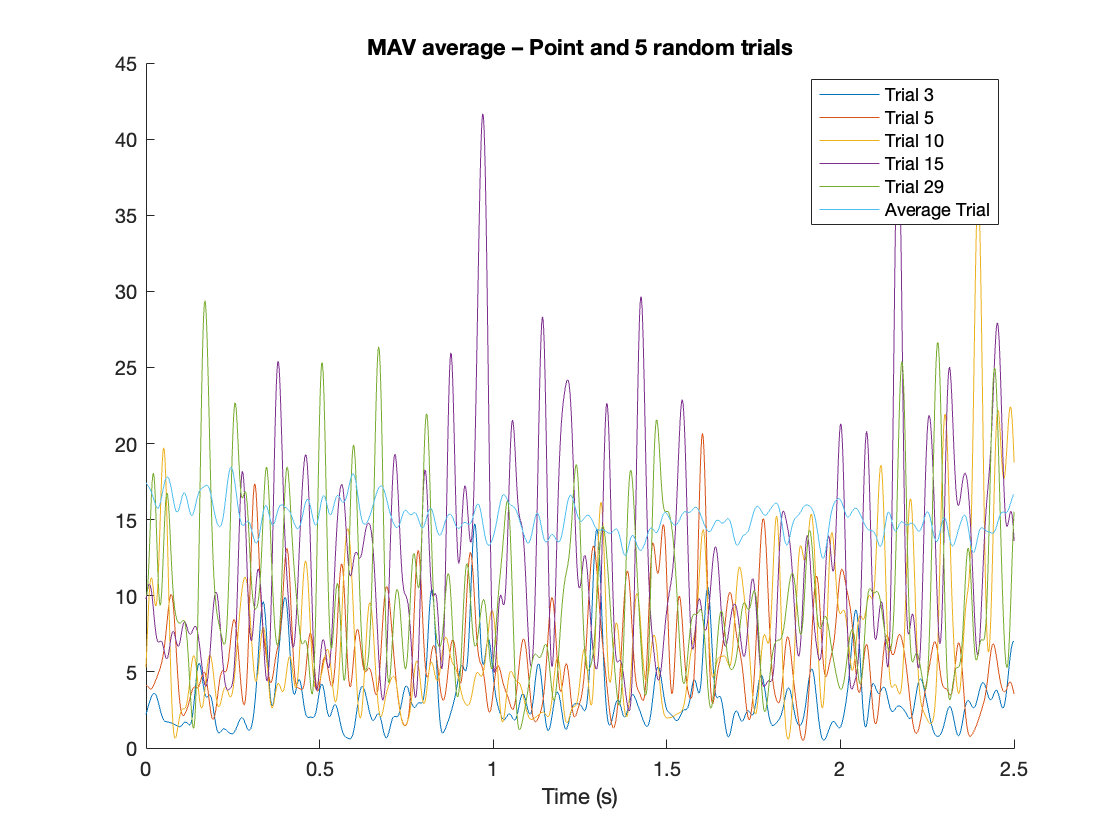
\includegraphics[width=0.9\textwidth]{point.png}
\end{center}

\section{Classification}
I used LDA and QDA as my classifiers. Using run-wise cross-validation lets us find the best runs to train on by holding out one run for validation. We can now predict classes for future runs. LDA classifiers performed best during cross-validation and we can see the accuracies below for each subject's sixth run. Additionally, the sixth run accuracies were generally a little worse than the cross validation accuracy, potentially because test accuracy can often be lower than validation accuracy due to overfitting of the training data.

\begin{center}
    \begin{tabular}{c c c c}
        \toprule
        Subject & LDA Accuracy \\ \midrule
        1 & 0.815 \\
        2 & 0.919 \\ \bottomrule
    \end{tabular}
\end{center}

We can also perform transfer decoding by testing the decoder of each subject on the sixth run of the other subject. We see that the accuracies are a lot which indicates that the data from one subject is not enough to generalize to the other subject.

\begin{center}
    \begin{tabular}{c c c c}
        \toprule
        Subject & LDA Accuracy \\ \midrule
        1 & 0.392 \\
        2 & 0.387 \\ \bottomrule
    \end{tabular}
\end{center}

The classification results are overall good for each subject. However, the classifiers don't generalize to other subjects well. We should try to collect more data from many different subjects and average across them to create a more robust classifier.

\end{document}